\documentclass[12pt, oneside]{article}
\usepackage{amsmath}
\usepackage[a4paper,margin=1cm,footskip=.5cm]{geometry}
\usepackage{amsfonts}
\usepackage{listings}
\usepackage{color}
\usepackage{graphicx}

\definecolor{mygreen}{rgb}{0,0.6,0}
\definecolor{mygray}{rgb}{0.5,0.5,0.5}
\definecolor{mymauve}{rgb}{0.58,0,0.82}

\lstset{ %
  backgroundcolor=\color{white},   % choose the background color; you must add \usepackage{color} or \usepackage{xcolor}
  basicstyle=\footnotesize,        % the size of the fonts that are used for the code
  breakatwhitespace=false,         % sets if automatic breaks should only happen at whitespace
  breaklines=true,                 % sets automatic line breaking
  captionpos=b,                    % sets the caption-position to bottom
  commentstyle=\color{mygreen},    % comment style
  deletekeywords={...},            % if you want to delete keywords from the given language
  escapeinside={\%*}{*)},          % if you want to add LaTeX within your code
  extendedchars=true,              % lets you use non-ASCII characters; for 8-bits encodings only, does not work with UTF-8
  frame=single,	                   % adds a frame around the code
  keepspaces=true,                 % keeps spaces in text, useful for keeping indentation of code (possibly needs columns=flexible)
  keywordstyle=\color{blue},       % keyword style
  language=R,                 % the language of the code
  otherkeywords={*,...},           % if you want to add more keywords to the set
  numbers=left,                    % where to put the line-numbers; possible values are (none, left, right)
  numbersep=5pt,                   % how far the line-numbers are from the code
  numberstyle=\tiny\color{mygray}, % the style that is used for the line-numbers
  rulecolor=\color{black},         % if not set, the frame-color may be changed on line-breaks within not-black text (e.g. comments (green here))
  showspaces=false,                % show spaces everywhere adding particular underscores; it overrides 'showstringspaces'
  showstringspaces=false,          % underline spaces within strings only
  showtabs=false,                  % show tabs within strings adding particular underscores
  stepnumber=2,                    % the step between two line-numbers. If it's 1, each line will be numbered
  stringstyle=\color{mymauve},     % string literal style
  tabsize=2,	                   % sets default tabsize to 2 spaces
  title=\lstname                   % show the filename of files included with \lstinputlisting; also try caption instead of title
}

\title{Preliminary Analysis}
\date{\today}

\begin{document}

\maketitle

\section{Distribution of correct answers}

\subsection{Code}
\begin{lstlisting}
## Test answer distribution
ans1 <- test$correctAnswer
table(ans1)/length(ans1)
# ans1
#        A         B         C         D 
# 0.2556515 0.2457269 0.2501378 0.2484837 

## Train answer distribution
ans2 <- train$correctAnswer
table(ans2)/length(ans2)
# ans2
#        A         B         C         D 
# 0.2556515 0.2457269 0.2501378 0.2484837

library('lattice')
x1 <- histogram(~correctAnswer, data=test,
          type="density",
          xlab="Answer",
          main = "Test")
x2 <- histogram(~correctAnswer, data=train,
          type="density",
          xlab="Answer",
          main = "Train")
require(gridExtra)
grid.arrange(x1, x2, ncol=2)
\end{lstlisting}

\subsection{Plots}
\begin{figure}[h]
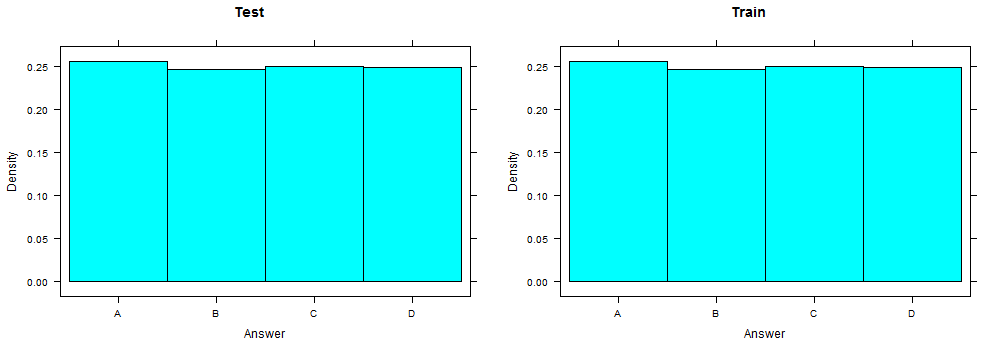
\includegraphics[scale=0.5]{./Plots/Rplot01.png}
\centering
\end{figure}

\section{Term Frequency}
\subsection{Code}
\begin{lstlisting}
library('tm')

# Build corpus
train_data.corpus <- Corpus(VectorSource(train$question))

# make each letter lowercase
train_data.corpus <- tm_map(train_data.corpus, tolower)

# remove punctuation 
train_data.corpus <- tm_map(train_data.corpus, removePunctuation)

# remove generic and custom stopwords
train_stopwords <- c(stopwords('english'))
train_data.corpus <- tm_map(train_data.corpus, removeWords, train_stopwords)

# build a term-document matrix
train_data.dtm <- TermDocumentMatrix(train_data.corpus)
train_data.dtm

# inspect most popular words (change lowfreq for lower bound)
findFreqTerms(train_data.dtm, lowfreq=50)
\end{lstlisting}

\begin{lstlisting}
# Most Frequent (>=50) Terms
  [1] "according"    "acid"         "algorithm"    "along"        "also"         "another"      "associated"  
  [8] "body"         "called"       "can"          "carbon"       "catalyst"     "cause"        "caused"      
 [15] "causes"       "cell"         "cells"        "certain"      "chemical"     "class"        "common"      
 [22] "complex"      "compound"     "compounds"    "constant"     "contains"     "create"       "created"     
 [29] "density"      "derivative"   "derived"      "described"    "developed"    "discovered"   "disease"     
 [36] "divided"      "due"          "effect"       "electron"     "element"      "elements"     "energy"      
 [43] "entities"     "enzyme"       "equal"        "equals"       "equation"     "experiment"   "factor"      
 [50] "field"        "first"        "form"         "formation"    "formed"       "forms"        "formula"     
 [57] "found"        "function"     "functional"   "functions"    "gene"         "given"        "gives"       
 [64] "group"        "high"         "include"      "involves"     "known"        "law"          "light"       
 [71] "like"         "magnetic"     "man"          "mass"         "material"     "may"          "mechanism"   
 [78] "metal"        "method"       "model"        "molecule"     "molecules"    "name"         "named"       
 [85] "namesake"     "negative"     "number"       "numbers"      "object"       "objects"      "occur"       
 [92] "occurs"       "often"        "one"          "ones"         "order"        "organ"        "paper"       
 [99] "part"         "particle"     "particles"    "pathway"      "phenomenon"   "phylum"       "potential"   
[106] "power"        "presence"     "pressure"     "problem"      "process"      "produce"      "produced"    
[113] "product"      "property"     "proportional" "proposed"     "protein"      "proteins"     "quantity"    
[120] "quantum"      "reaction"     "region"       "related"      "result"       "results"      "rule"        
[127] "set"          "showed"       "solution"     "sometimes"    "space"        "square"       "state"       
[134] "states"       "step"         "structure"    "structures"   "study"        "substance"    "substances"  
[141] "surface"      "syndrome"     "synthesis"    "system"       "systems"      "technique"    "temperature" 
[148] "term"         "theorem"      "theory"       "three"        "time"         "times"        "two"         
[155] "type"         "types"        "use"          "used"         "uses"         "using"        "value"       
[162] "variety"      "version"      "via"          "water"        "whose"        "work"  
\end{lstlisting}

\section{Word Associations}
\begin{lstlisting}
## Example: Associations with the word "cells", lower bound on correlation 0.2
findAssocs(train_data.dtm, 'cells', 0.20)
           cells
glial       0.33
purkinje    0.32
schwann     0.27
amacrine    0.26
epithelial  0.23
# Note association score is percentage that term occurs with the search term (i.e. "glial" occurs with "cells" 33% of the time)
\end{lstlisting}

\section{Clustering}

\subsection{Code}
\begin{lstlisting}
# http://www.statmethods.net/advstats/cluster.html (Robert I. Kabacof’s “Cluster Analysis” )

# remove sparse terms = simpler cluster plot (need to think about this in terms of classifying question types)
train_data.dtm2 <- removeSparseTerms(train_data.dtm, sparse=0.95)

# convert the sparse term-document matrix to a standard data frame
train_data.df <- as.data.frame(inspect(train_data.dtm2))

# inspect dimensions of the data frame
nrow(train_data.df)
ncol(train_data.df)

train_data.df.scale <- scale(train_data.df)
d <- dist(train_data.df.scale, method = "euclidean") # distance matrix
fit <- hclust(d, method="ward")
plot(fit) # display dendogram? (i.e. 1-gram)

groups <- cutree(fit, k=5) # cut tree into 5 clusters
# draw dendogram with red borders around the 5 clusters
rect.hclust(fit, k=5, border="red")
\end{lstlisting}

\subsection{Plot}
\begin{figure}[h]
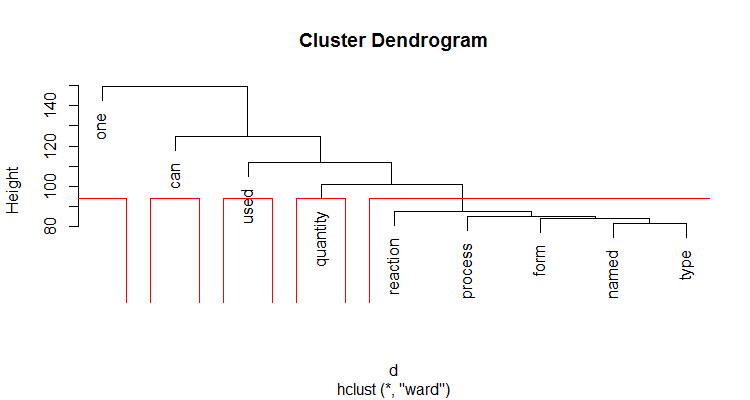
\includegraphics[scale=0.5]{./Plots/Rplot02.png}
\centering
\caption{More popular terms are higher up, while more associated terms are closer together}
\end{figure}

\end{document}